\chapter{Architektur  \label{chap_archtitektur}}
Die Netzwerkarchitektur von \ac{ITS} Stations umfasst sowohl interne als auch externe Netzwerke. Laut Standard \cite{etsi302636-3}, bzw. Standard \cite{etsi102636-3} sind dabei folgende externe Netzwerke erfasst:

\begin{itemize}
 	\item ITS ad hoc network.
	\item Access network (ITS access network, public access network, private access network).
	\item Core network (e.g. the Internet).
\end{itemize}

Auf der Grafik \ref{fig:architektur_ueberblickNetzwerke} sind die verschiedenen Netzwerke visualisiert. Diese Art der Darstellung entspricht der höchsten Abstraktionsebene. Die verschiedenen Netzwerke sind in der Grafik als Wolken dargestellt. Neben den Netzwerken sind auch die Verbindungen visualisiert.


Zusätzlich zu den hier beschriebenen Netzwerken kann eine \ac{ITS} Station ein eigenes Netzwerk, das die Teilkomponenten der \ac{ITS} Station verbindet, betreiben. Die verschiedenen Netzwerke werden benötigt, damit alle Dienste mit ihren verschiedenen Anforderungen bedient werden können.

\begin{figure}[h]
	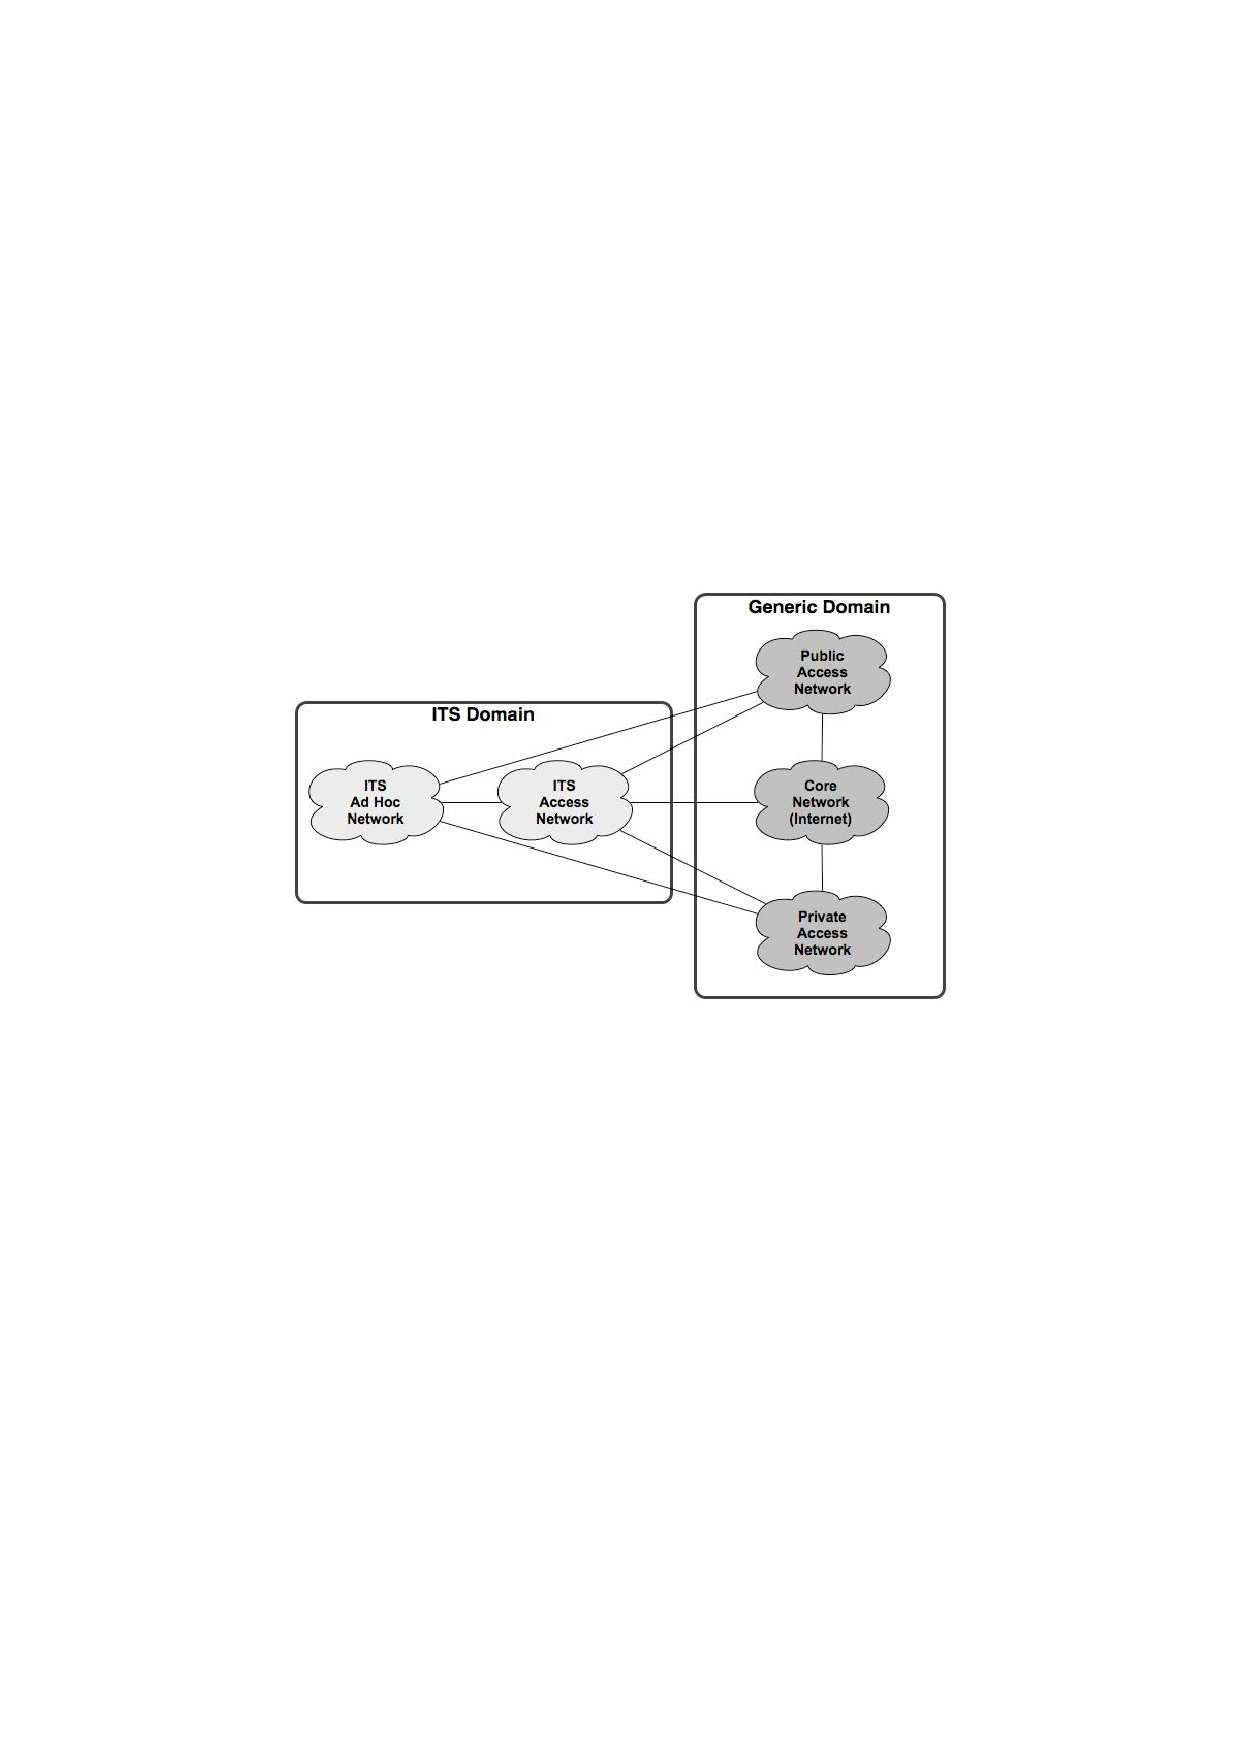
\includegraphics[width=0.99\textwidth]{content/images/02_architektur/uebersichtExterneNetzwerke.pdf}
	\caption{Überblick über die externen Netzwerke \cite{etsi302636-3}}
	\label{fig:architektur_ueberblickNetzwerke}
\end{figure}

\section{Übersicht über die verschiedenen Netzwerke}
Dieser Abschnitt soll lediglich eine Übersicht über die verwendeten Netzwerke geben. Eine weitere Erklärung der Netzwerke findet an dieser Stelle nicht statt und ist nicht Gegenstand dieser Ausarbeitung. Die Netzwerke dürfen auch nicht isoliert betrachtet werden. Im Abschnitt \ref{funktionsweise_funktionaleKomponenten} wurden funktionale Komponenten mit Routingfunktionalitäten vorgestellt. Diese können die Netze und somit ihre Vorteile, bzw. ihre Dienste, miteinander verbinden.

Selbstverständlich benötigen die \ac{ITS} Stations Zugang zu einem der im Folgenden aufgeführten Netze. Der Zugang zum Core Network \ref{achitektur_coreNetwork} erfolgt über eins der anderen Netze. 

\subsection{ITS Ad Hoc Network\label{achitektur_adHocNetwork}}
Das \ac{ITS} Ad Hoc Netzwerk ist das Netzwerk für die Kommunikation zwischen \ac{IRS}, \ac{IVS} und \ac{PSS}. Die Kommunikation findet über die Luftschnittstelle statt. Sie ist in ihrer Reichweite begrenzt, dafür ist sie mobil einsetzbar. Die Drahtlose Kommunikation wird im Normalfall über den Standard ITS-G5 ermöglicht.


\subsection{ITS Access Network \label{architektur_itsAccessNetwork}}
\tocheck{Nicht die blasseste Ahnung ob das mit den Access Networks stimmt}
ITS Access Network werden zur Vernetzung von \ac{ITS} Komponenten verwendet. Diese Netzwerke bieten den Zugang für die entsprechenden \ac{ITS} Services. Sie werden als eigene Netzwerke realisiert. \ac{ITS} Stations werden durch Access Networks verbunden. Das bedeutet, dass \ac{IRS} untereinander über Access Networks verbunden sein können, es können aber auch Stations, die normalerweise Ad Hoc miteinander kommunizieren dieses Netz nutzen. 

\subsection{Public Access Network}
Ein Public Access Network ermöglicht den Zugang in öffentlich zugängliche Mehrzwecknetzwerke. Dieses Netzwerk kann beispielsweise dazu genutzt werden, um \ac{ITS} Stations mit dem Core Netzwerk zu verbinden. 

\subsection{Private Access Network}
Ein Private Access Network reguliert den Zugang durch die Teilnehmer. Die angebotenen Datendienste stehen nur einer bestimmten Gruppe von Nutzern zur Verfügung. Mit Private Access Networks besteht die Möglichkeit, eine gesicherte Verbindung in ein anderes Netzwerk aufzubauen. So kann beispielsweise ein \ac{IVS} auf das Intranet einer Firma zugreifen. 

\subsection{Core Network \label{achitektur_coreNetwork}}
Das Core Network ist ein Verbindungsnetz. Es hat keine \ac{ITS} Funktionalitäten und wird im Standard auch nicht weiter spezifiziert. Es wird in Verbindung mit den Public Access Network dazu genutzt, traditionelle Dienste, wie Internet oder Email, anzubieten.
 
\begin{figure}
	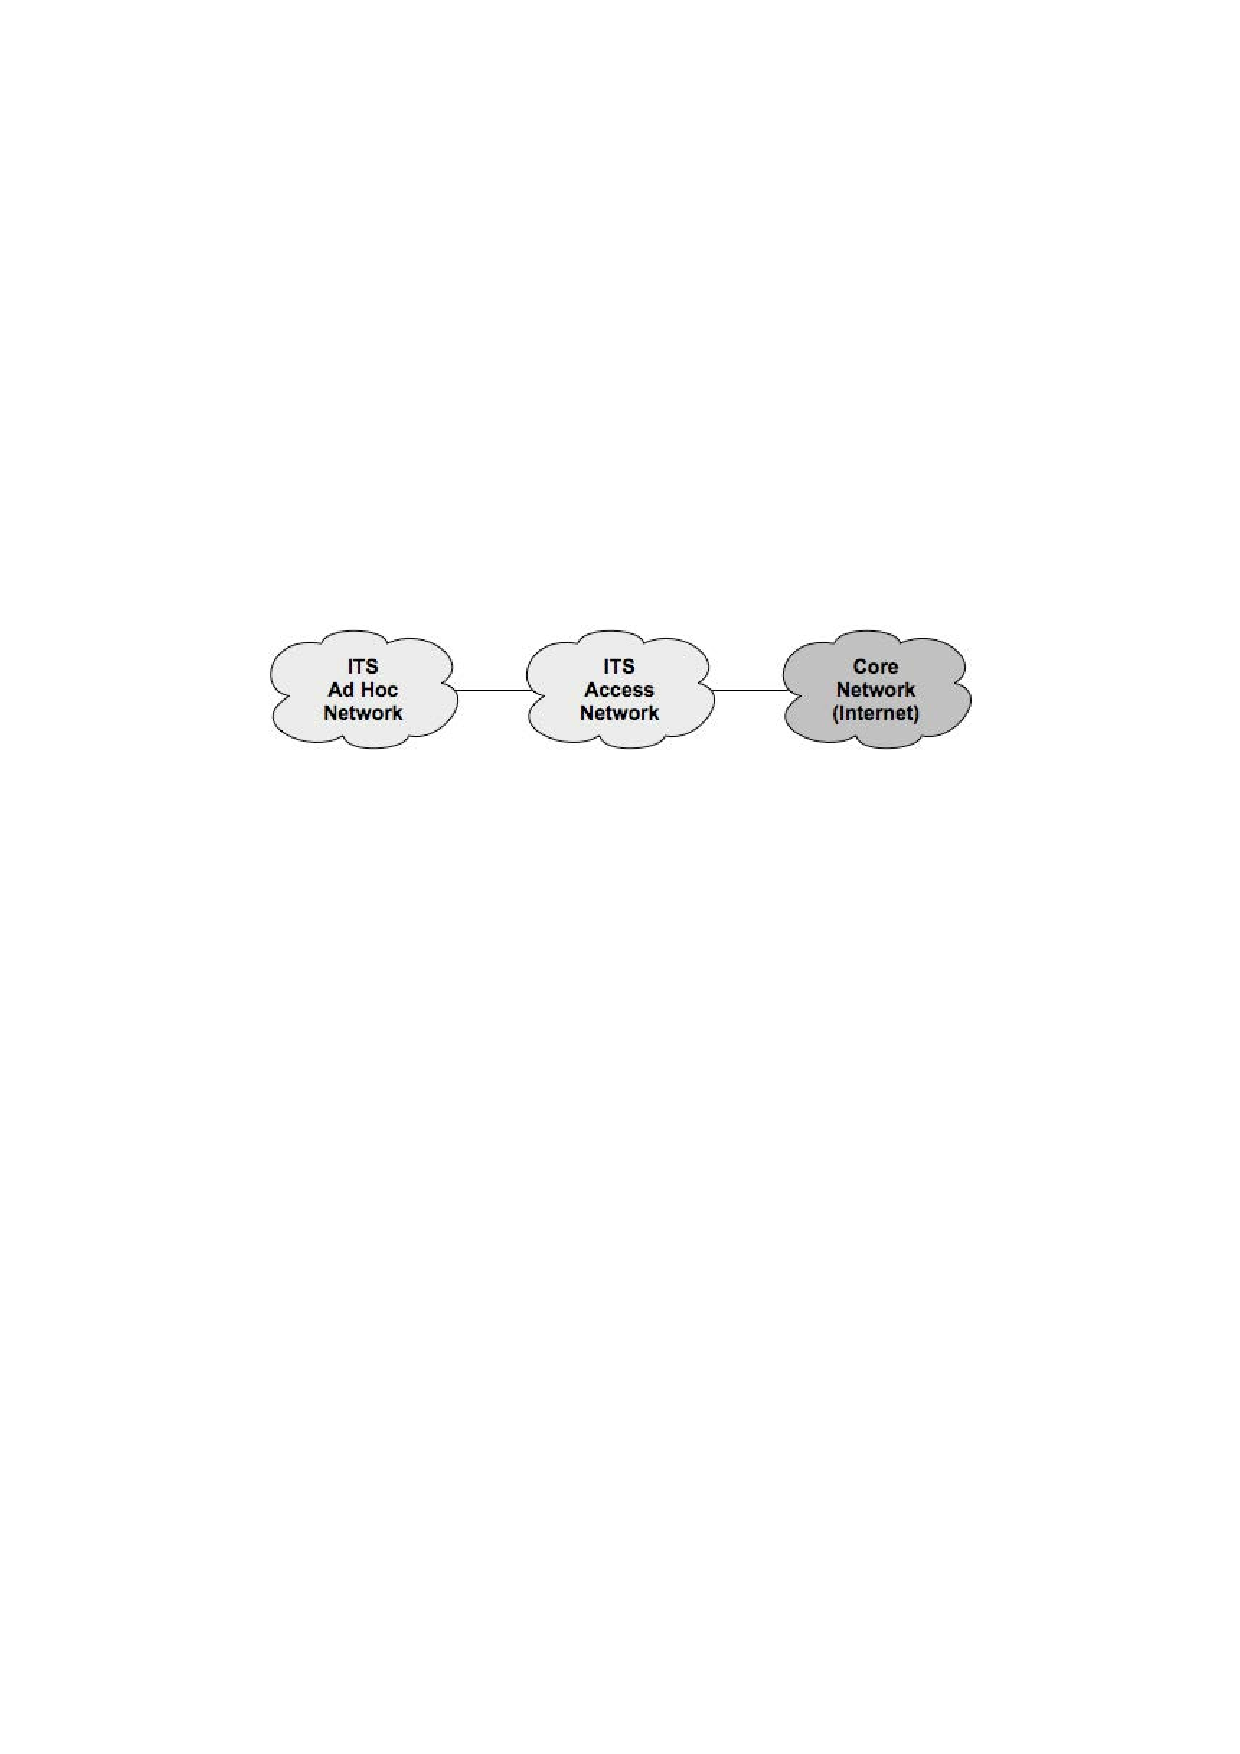
\includegraphics[width=0.75\textwidth]{content/images/02_architektur/netzwerkSzenario.pdf}
	%\vspace{2cm}
	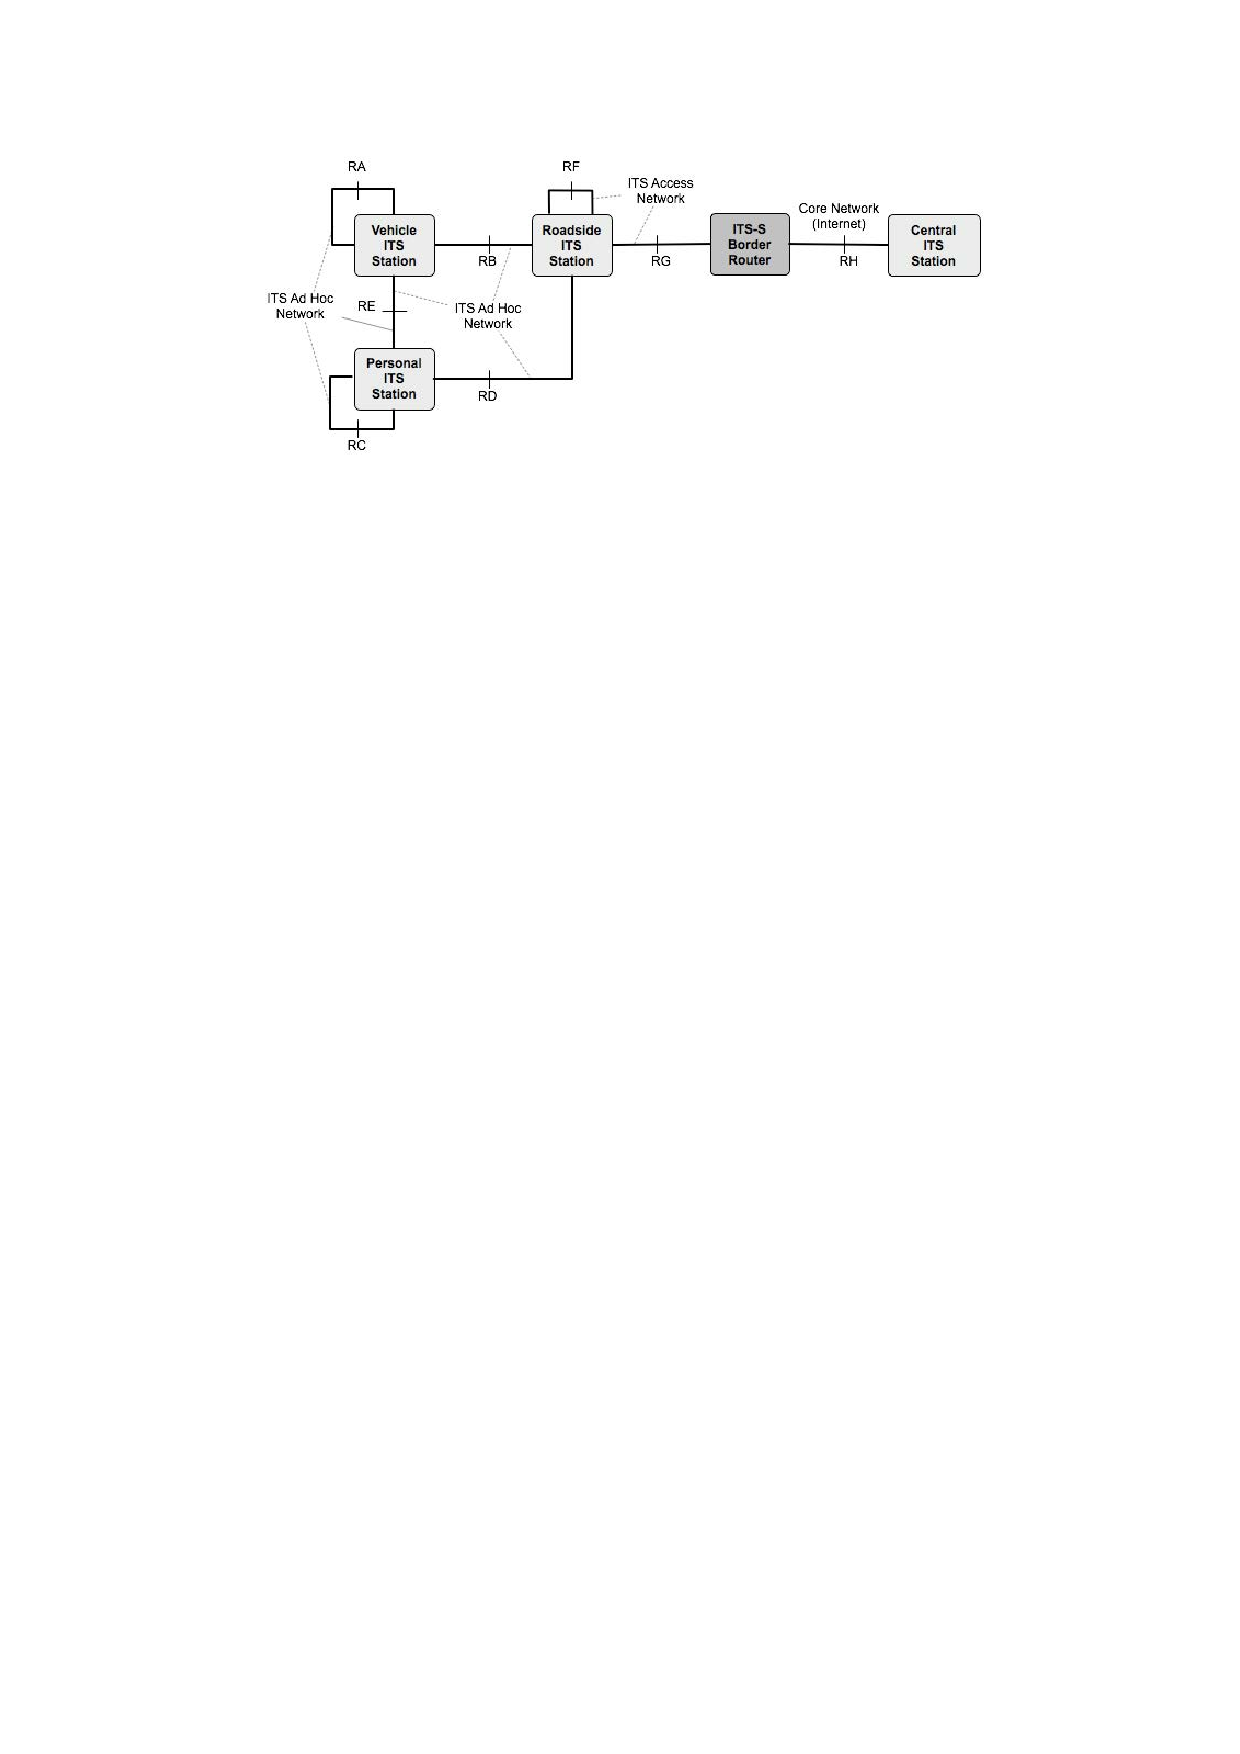
\includegraphics[width=0.75\textwidth]{content/images/02_architektur/verbindungenNetzwerkSzenario.pdf}
	\caption{Netzwerkszenario mit dazugehöriger Implementierung \cite{etsi302636-3}}
	\label{fig:architektur_netzwerkSzenario}
\end{figure}

Die Grafik \ref{fig:architektur_netzwerkSzenario} stammt aus dem Standard \cite{etsi302636-3}. Dort ist im oberen Teil der Grafik ein Szenario beschrieben, welche Netzwerke miteinander verbunden sein können.  Zu erkennen ist, dass die Netzwerke ITS Ad Hoc Netzwerk \ref{achitektur_adHocNetwork}, ITS Access Network \ref{architektur_itsAccessNetwork} und das Core Network  \ref{achitektur_coreNetwork} miteinander verbunden sein sollen.

Der untere Teil der Grafik zeigt eine Implementierungsmöglichkeit dieses Szenarios. Die hellen Rechtecke beschreiben die Komponenten, die in dieser Implementierung im System integriert sind, das dunkle Rechteck beschreibt die funktionale Komponente, die in diesem System beteiligt ist. Die Linien sind mit dem Typ des Netzwerks, welches sie repräsentieren beschriftet und zusätzlich mit dem Network Reference Point, den sie benutzen, beschriftet.
\todo{Sollen wir hier noch was zum Thema Network Reference Point schreiben? Ich glaube aber, dass die noch in den Layern kommen}


Auflistung und kurze Beschreibung der genutzten Network Reference Points:
\begin{itemize}
	\item \textbf{RA: } Reference Point zwischen \ac{IVS} über das ITS Ad Hoc Network
	\item \textbf{RB: } Reference Point zwischen \ac{IVS} und \ac{IRS} über das ITS Ad Hoc Network
	\item \textbf{RC: } Reference Point zwischen \ac{PSS} über das ITS Ad Hoc Network
	\item \textbf{RD: } Reference Point zwischen \ac{PSS} und \ac{IRS} über das ITS Ad Hoc Network
	\item \textbf{RE: } Reference Point zwischen \ac{IVS} und \ac{PSS} über das ITS Ad Hoc Network
	\item \textbf{RF: } Reference Point zwischen \ac{IRS} über das ITS Access Network
	\item \textbf{RG: } Reference Point zwischen \ac{IRS} und einem ITS-S Border Router \footnote{Der Border Router muss nicht explizit aufgeführt werden, da er als funktionale Komponente Teil einer Komponente ist. \label{ftn:borderRouter}} über das ITS Access Network 
	\item \textbf{RH: } Reference Point zwischen \ac{ICS} und ITS-S Border Router \footref{ftn:borderRouter} über das Core Network		
\end{itemize}

Erkennbar ist in dieser Implementierung, dass sich für mobile Stations Ad Hoc Netzwerke verwendet wurden. Diese haben den Vorteil, dass sie bereits in der Spezifikation mit der Luftschnittstelle ITS-G5 ausgestattet sind, was eine Mobilität erst ermöglicht. Was auch erkennbar ist, ist, dass die reinen ITS Netzwerke durch einen Border Router vom Core Network getrennt sind. Auch wenn hier nicht explizit aufgeführt, die \ac{ICS} benötigt in diesem Fall auch einen Border Router.

 
\section{ITS Station Reference Architecture}
Eine Referenzarchitektur beschreibt ein allgemeines Modell einer Architektur. Das bedeutet, dass basierend auf dieser Architektur verschiedene Implementierungen existieren können. 

Die \ac{ITS} Station Reference Architecture unterscheidet sich grundlegend von bekannten Architekturen. Da sie während der Entwicklung an das \ac{OSI} Modell angelehnt war, ergeben sich einige Parallelen:
\begin{itemize}
	\item Trennung der einzelnen Layer
	\item Definition von Service Primitiven zwischen den Layern
	\item Die Standards beziehen die Layer auf die \ac{OSI} Layer. 
\end{itemize}


Obwohl das \ac{ITS} Station Reference Protocol bei der Entwicklung an das \ac{OSI} Modell angelehnt wurde gibt es jedoch einen gravierenden Unterschied: In der \ac{ITS} Station Reference Architecture sind Cross Layer vorgesehen. Das \ac{OSI} Referenzmodell ist wasserfallartig aufgebaut. Das bedeutet, dass die einzelnen Layer übereinander angeordnet sind. Jeder Layer hat jeweils nur zu dem direkt über- und unterliegenden Layer eine Schnittstelle. Cross Layer sind Layer, die in mehrere dieser Schichten Schnittstellen haben. Sie erweitern die vorhanden Layer in horizontaler Richtung. Im Fall der \ac{ITS} Station Reference Architecture sind das die Layer \glqq Management\grqq~ und \glqq Security\grqq. Sie haben Schnittstellen, bzw. Primitiven in alle anderen Layer. 

\begin{figure}
	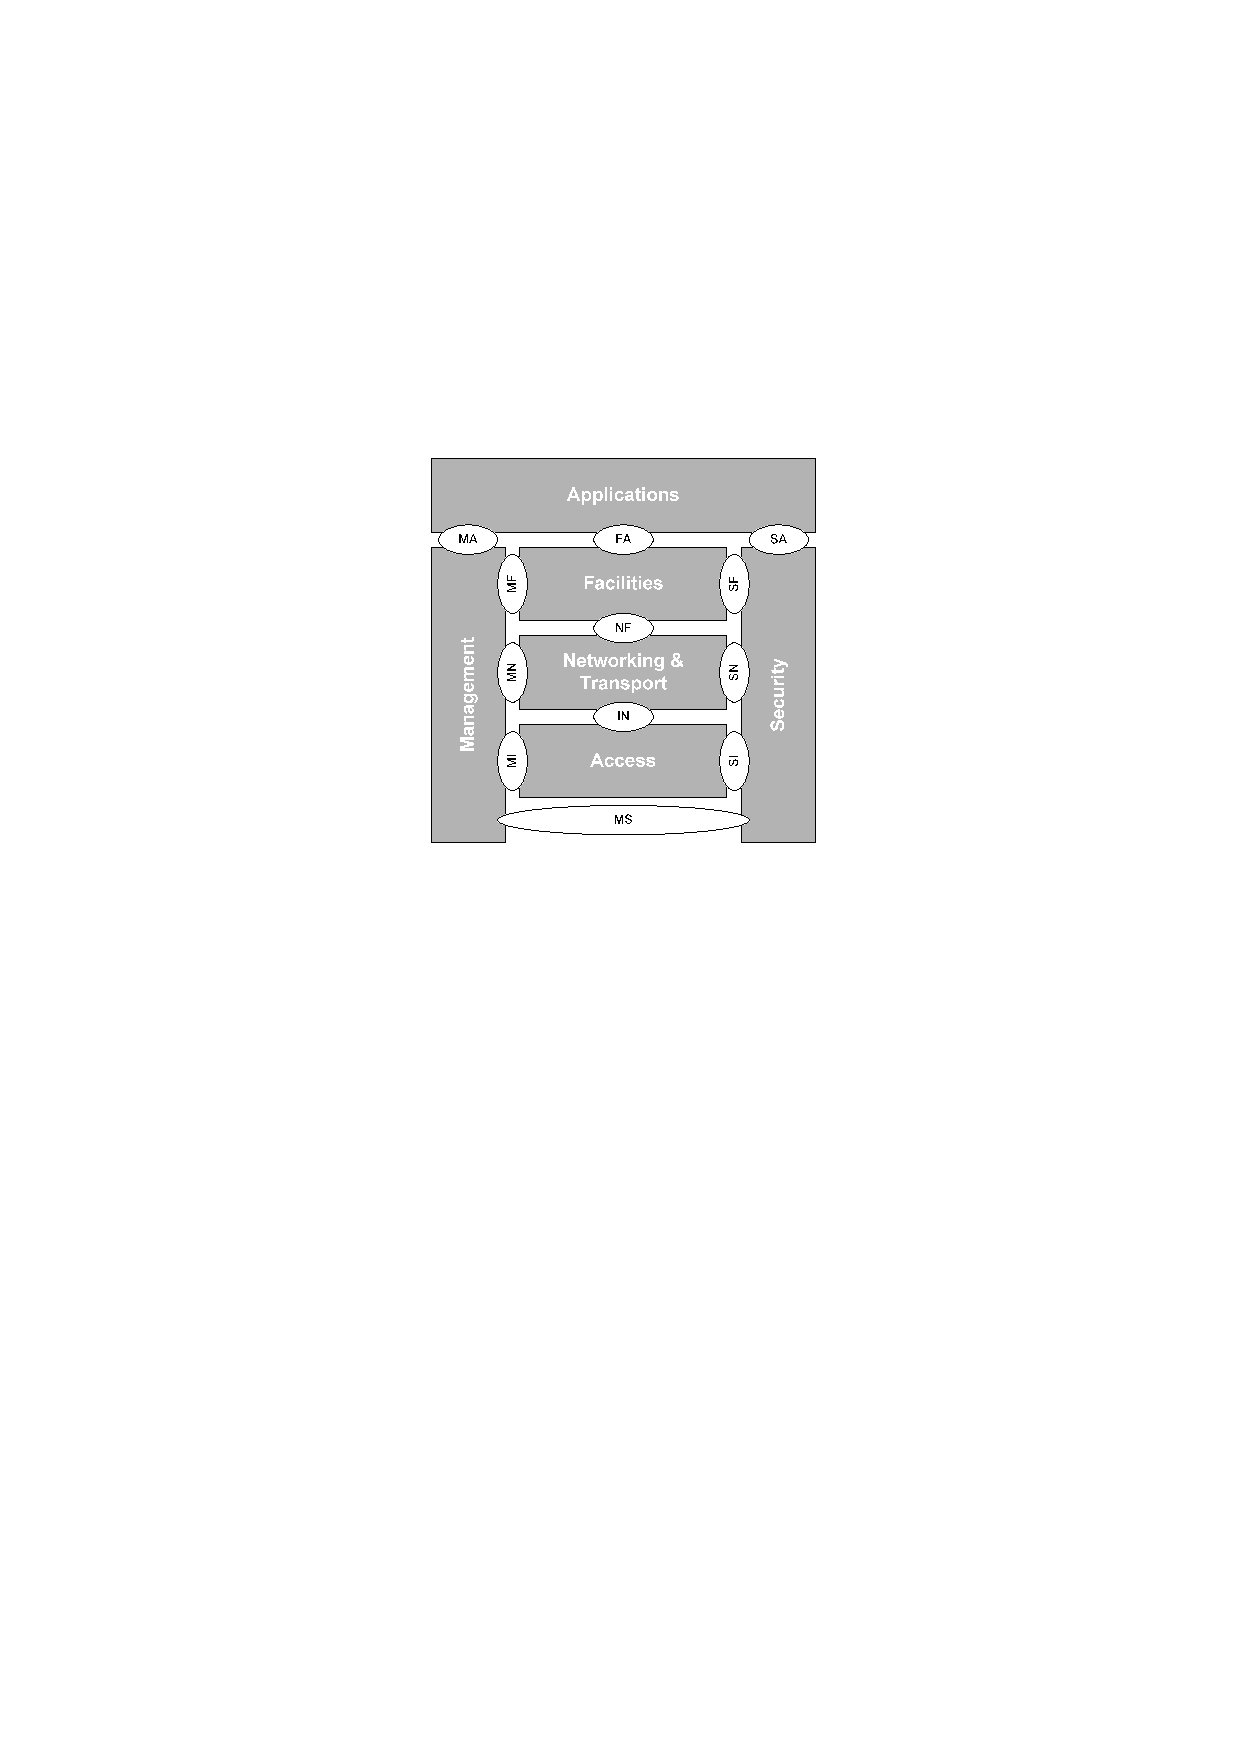
\includegraphics[width=0.75\textwidth]{content/images/02_architektur/stationReferenceArchitecture.pdf}
	\caption{Darstellung der ITS Station Reference Architecture \cite{etsi2010302}}
	\label{fig:funktionsweise_referenceArchitecture}
\end{figure}

\section{Wasserfall Layer}
Dieser Abschnitt beschreibt die Layer, die klassisch übereinander angeordnet sind. 

\subsection{Access}
Der Access Layer entspricht den \ac{OSI} Layern 1 und 2. 

\subsection{Networking \& Transporting}
Der Networking \& Transporting Layer entspricht den \ac{OSI} Layern 3 und 4.

\subsection{Facilities}
Der Facilities Layer entspricht den \ac{OSI} Layern 5, 6 und 7

\subsection{Applications}


\section{Cross Layer}
\subsection{Management Layer}
Beschrieben in \cite{etsi102723-2}
\todo{Management Layer genauer beschreiben}

\subsection{Security Layer}


\section{Data Security}

\section{Verwendete Protokolle}



